\documentclass{article}
\usepackage{amsfonts, amsmath, amssymb, amsthm} % Math notations imported
\usepackage{enumitem}
\usepackage[margin=1in]{geometry}
\usepackage{graphicx}
\graphicspath{ {./images/} }

\newtheorem{thm}{Theorem}
\newtheorem{prop}[thm]{Proposition}
\newtheorem{cor}[thm]{Corollary}

% title information
\title{Math 170A HW1}
\author{Neo Lee}
\date{04/07/2023}

% main content
\begin{document} 

% placing title information; comment out if using fancyhdr
\maketitle 

\textbf{Problem 1.} Done.
\bigbreak

\textbf{Problem 2.} Done.
\bigbreak

\textbf{Problem 3.} 
Figure 1 is the function that implements $ABx$ through $(AB)x$: 
\begin{figure}[h]
    \centering
    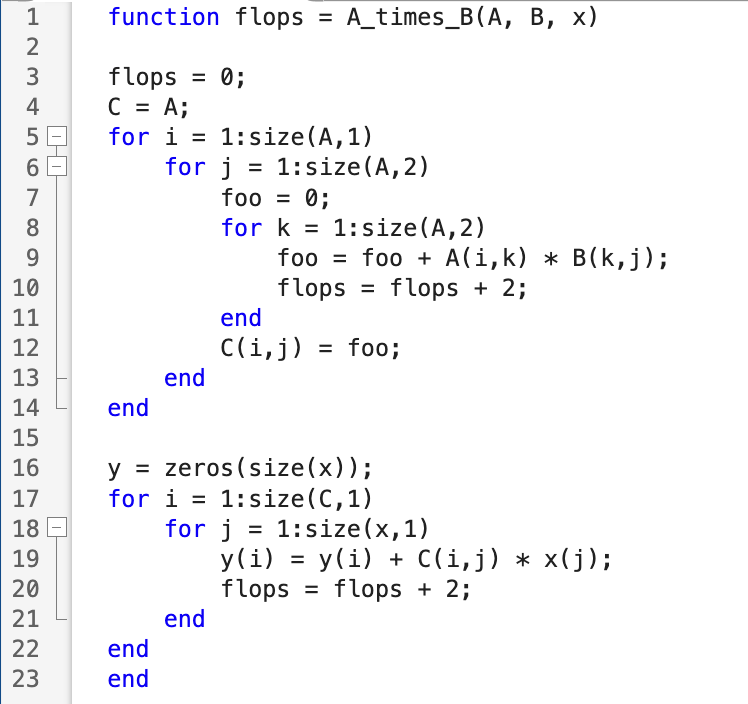
\includegraphics[scale = 0.5]{A_times_B_function.png}
    \caption{$(AB)\vec{x}$ function}
\end{figure}

Figure 2 shows the flop count for the function:
\begin{figure}[h]
    \centering
    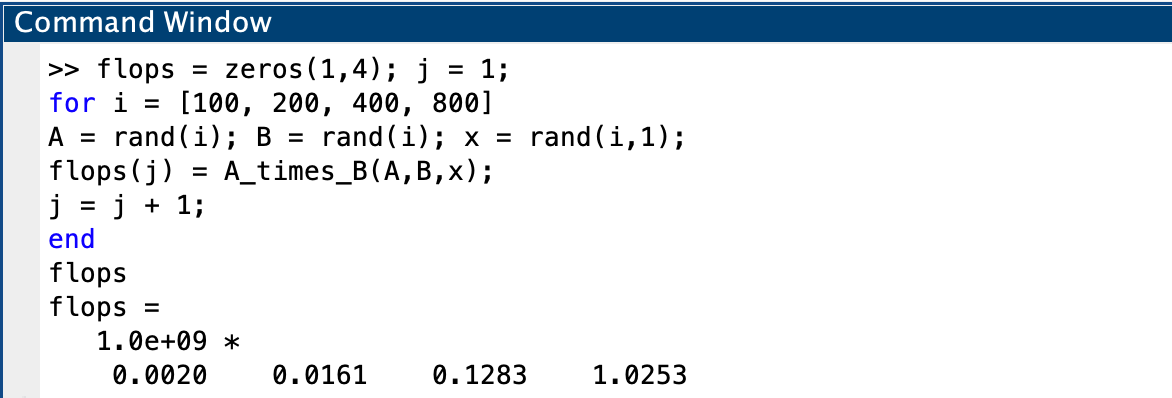
\includegraphics[scale = 0.5]{A_times_B_flops.png}
    \caption{Flop count for $(AB)\vec{x}$ function}
\end{figure}
\pagebreak

Figure 3 is the function that implements $AB\vec{x}$ through $A(B\vec{x})$:
\begin{figure}[h]
    \centering
    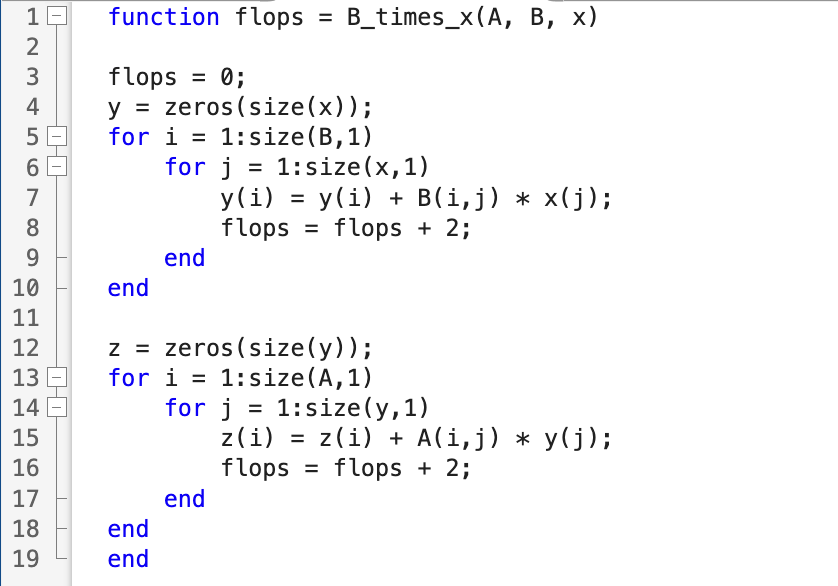
\includegraphics[scale = 0.5]{B_times_x_function.png}
    \caption{$A(B\vec{x})$ function}
\end{figure}

Figure 4 shows the flop count for the function:
\begin{figure}[h]
    \centering
    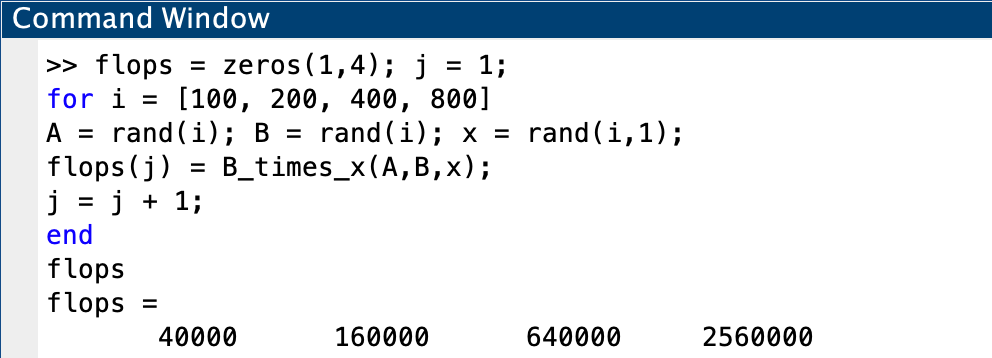
\includegraphics[scale = 0.5]{B_times_x_flops.png}
    \caption{Flop count for $A(B\vec{x})$ function}
\end{figure}

We can see apparently that the implementation of $A(B\vec{x})$ uses significantly fewer flops.

It is because assuming $n \times n$ matrix $A$ and $B$, the total number flops for $AB$ is $2n^3$.
Atfter computing $C = AB$, we need to multiply $C$ with $\vec{x}$, which requires another $2n^2$ flops. 
Hence, $(AB)\vec{x}$ requires $2n^3 + 2n^2$ flops in total with time complexity $O(n^3)$.

On the other hand, $\vec{z} = A(B\vec{x})$ requires $2n^2$ flops to compute $\vec{y} = B\vec{x}$, and $2n^2$ flops to compute $\vec{z} = A\vec{y}$.
Hence, in total $A(B\vec{x})$ requires only $4n^2$ flops with time complexity $O(n^2)$.
\bigbreak

\textbf{Problem 4.}
\begin{enumerate}[label=(\alph*)]
    \item 
    \begin{itemize}
        \item 5-th line initializes matrix $Z$ of dimension $m\times m$ with all entries equal 0.
        \item 6-th line initializes diagonal matrix $D$ of dimension $m\times m$ with diagonal entries equal to $m$.
        \item 7-th line initializes subdiagonal matrix $subD$ of dimension $m\times m$ with subdiagonal entries equal to $m$.
        \item 8-th line creates a matrix $A$ of dimension $m\times m$ with diagonal entries equal to $m$ and subdiagonal entries equal to $-m$. (Note: $A = D - subD;$ would do the same work.)
        \item 10-th line initializes a row vector $\vec{v}$ with $m$ elements, which each neighboring element differ by $\frac{1}{m}$.
        \item 11-th line creates a vector $\vec{b}$ by squaring each entry of $\vec{v}$, followed by transposing it to a column vector. It represents right hand side of the equation $x^2$ at each step interval.
        \item 13-th line solve the linear system $A\vec{u}=\vec{b}$ to find $\vec{u}$, which is a vector of all the approximations of $u(x)$ at each step interval.
        \item 15-th to 18-th lines plot the analytic solution to the ODE, $u(x) = \frac{x^3}{3}$, by plotting the value of $\frac{x^3}{3}$ at 100 equally separated points between 0 and 1.
        \item 20-th to 24-th lines plot the approximated solution to the ODE at $m$ equally separated points between 0 and 1.
    \end{itemize}
    
    \item 
    Figure 5 shows the plot of $solve\_ODE$ for $m=3,10,50$:
    \begin{figure}[h!]
        \centering
        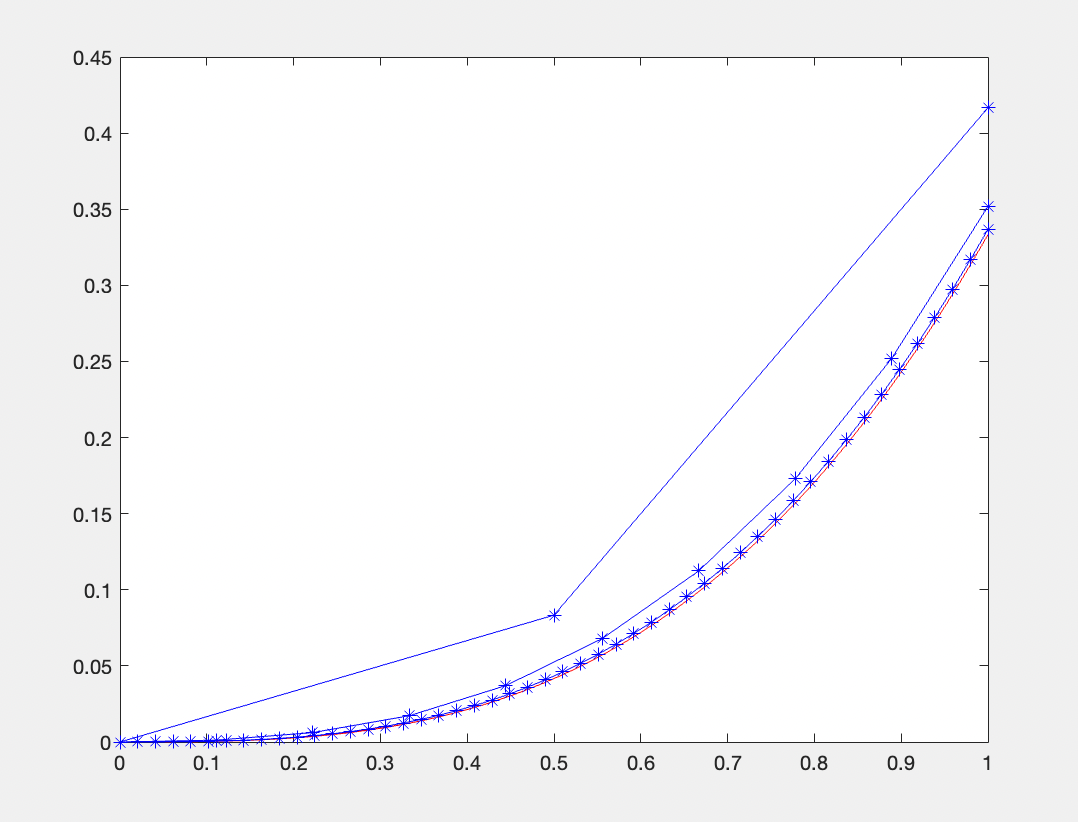
\includegraphics[scale = 0.5]{solve_ODE_plot.png}
        \caption{Plot of $solve\_ODE$}
    \end{figure}
    
    We can see the blue curve gets closer and closer to the red curve as $m$ increases, which means the approximation is getting closer and closer to the analytic solution.
    It is because as the interval $m$ gets smaller, the approximation gets more accurate.
    This agrees with the finite forward difference approximation where $u'(x) \approx \frac{u(x+\frac{1}{m}-u(x))}{\frac{1}{m}}$, and when $m$ gets bigger, the approximation is more accurate.
\end{enumerate}
\bigbreak

\textbf{Problem 5.}


\end{document}